% Drawing 154/05-16 -- folder 154, batch 05, archive page 93 (PDF page 94).
% Transcription: la moitié supérieure de la page est un grand dessin en couleur : deux droites horizontales vert clair, et entre elles une ligne médiane en tirets rouges marquée de petits traits bleus ; quatre droites verticales vert clair ; des droites orange qui, entre les verticales, se croisent sur la ligne médiane en forme de sabliers ou de losanges, et deux grands arcs orange, en haut et en bas, qui se croisent sur les verticales. Aux croisements du haut, trois petites marques étiquetées $\nu$, $\nu'$ et $\nu'$, avec des arcs en tirets vert clair. Deux légendes sur la droite horizontale du haut : « $n - \nu$ » et « $n - 1 - (\nu - 1) - (\nu' - 1)$ »
% Kind: strip between two lines: hourglasses on a dashed median. Method 2 (schematic redraw from the facsimile). Status: ok.
% Notes: Four light green verticals, two light green horizontals, the red dashed median with a short blue tick near each vertical; the wavy orange curve at the top and its mirror at the bottom, each crossing the verticals, with a lens (two arcs and a chord) between the second and third verticals and short crossing strokes at the first and fourth; between the verticals, orange lines from the top wave to the bottom wave: plain ones, and four hourglasses whose two sides start from one point of the top wave, meet the upper horizontal, cross on the median, meet the lower horizontal and join again on the bottom wave. The hourglasses are drawn from seven computed points each; the extra strokes inside the second and fourth, and the narrow kinked one right of the third vertical, are simplified. The three labels at the top crossings are placed after the transcription (nu, nu', nu'); the dashed light green arcs beside them are drawn at the four crossings; the two legends are on the upper horizontal. Redrawn 2026-11-12 (issue 128): to check again. 2026-11-14, Claude Opus 5.5, overlay check (issue 147): rasterised from its own coordinates over the 400 dpi colour scan on a unit grid, measured against the colour masks of the ink, corrected and laid over it again; not compiled (no TeX in the session). The simplified hourglasses are redrawn stroke by stroke from the scan. Second (x 36 to 46): three strokes leave the top point on the upper wave, the left side to the upper horizontal and on through the crossing on the median to the lower right corner, the right side bowed outwards to the upper horizontal and on to the lower left corner, and a middle stroke straight down through the crossing to the bottom point; from the two lower corners two strokes run to the bottom point, where the three strokes cross and run on a little below the wave. Third (x 62 to 67, the narrow kinked one): two strokes from the top point, one to the upper horizontal at the left corner and down through the crossing, then straight down to the bottom wave, the other straight down to the upper horizontal and on through the crossing to the lower left corner; a third stroke from below that corner to the bottom point and below the wave. Fourth (x 70 to 78): the left side to the upper horizontal and through the crossing to the lower right corner, the right side to the upper horizontal, through the crossing to the lower left corner and down to the bottom point, a middle stroke from the top through the crossing that stops under the lower horizontal, and two strokes from under the lower horizontal (one from the right corner, one from the middle) to the bottom point. At every hourglass the strokes cross at the top and bottom points and run on 1.5 to 2 units beyond the wave, as on the page; the plain strokes are moved onto the middle of their ink (by up to 1 unit) and end where their ink ends. Every orange, green, red and blue stroke now lies on its ink to within about 1 unit. Left out: the faint pencil underdrawing beside some orange strokes. Status set to ok.
% Coordinates: 1 unit = 1 mm = 1/100 of the crop width (bbox in page fractions: [0.155, 0.1, 0.925, 0.36]).
% Redrawn by Claude (claude-fable-5-2), issue #128, 2026-11-12; not checked by a human; not compiled (no TeX in the session).
% Checked by Claude (claude-opus-5-5) 2026-11-14 (issue #147): overlaid on the 400 dpi colour facsimile, corrected; not compiled (no TeX in the session). Not checked by a human. Status: ok.
% Rights: reproduces part of the work -- behind RENDER_TRANSCRIPTS, never published by itself.
\documentclass[tikz,border=3pt]{standalone}
\usepackage{amsmath,amssymb}
\usetikzlibrary{patterns,arrows.meta}
\tikzset{Or/.style={orange!90!black}, Lg/.style={green!60!black!70}, Rd/.style={red!85!black}, Bl/.style={blue!70!black}, pencil/.style={black!45}, struck/.style={black!35}, mpt/.style={circle,draw,inner sep=1.3pt}, pt/.style={circle,fill,inner sep=0.9pt}, opt/.style={circle,draw,fill=white,inner sep=1.1pt}}
\begin{document}
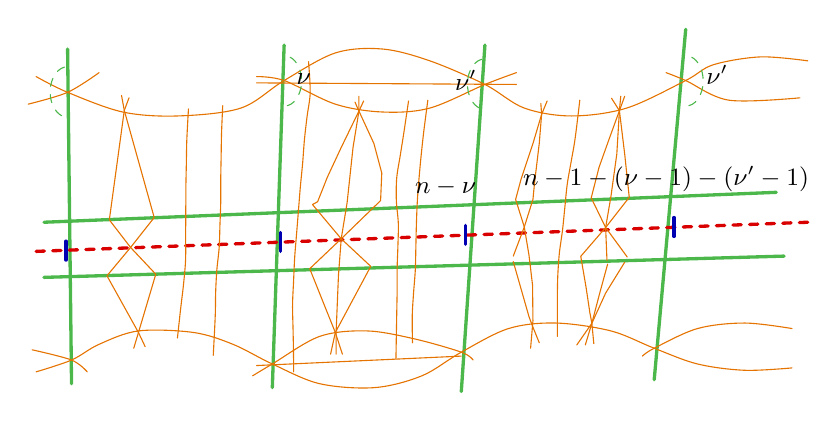
\begin{tikzpicture}[x=1mm,y=1mm,line cap=round,line join=round,font=\scriptsize]
\draw[Lg,very thick] (6,-3) -- (6.5,-45.5);
\draw[Lg,very thick] (33.5,-2.5) -- (32,-46);
\draw[Lg,very thick] (59,-2.5) -- (56,-46.5);
\draw[Lg,very thick] (84.5,-0.5) -- (80.5,-45);
\draw[Lg,very thick] (3,-25) -- (96,-21.2);
\draw[Lg,very thick] (3,-32) -- (97,-29.3);
\draw[Rd,dashed,very thick] (2,-28.7) -- (100,-25);
\draw[Bl,very thick] (5.8,-27.4) -- (5.8,-29.8);
\draw[Bl,very thick] (33,-26.3) -- (33,-28.7);
\draw[Bl,very thick] (56.5,-25.4) -- (56.5,-27.8);
\draw[Bl,very thick] (83,-24.4) -- (83,-26.8);
\draw[Or] plot[smooth, tension=0.55] coordinates {(2,-6.5) (6,-8.5) (13,-11) (20,-11.5) (28,-10.5) (33.5,-7) (40,-3.5) (46,-3) (52,-4.5) (59,-7.5) (64,-10.5) (70,-11.5) (77,-10.5) (84.5,-7) (88,-5) (94,-4) (100,-4.5)};
\draw[Or] plot[smooth, tension=0.55] coordinates {(1,-10) (6,-8.5) (10,-6)};
\draw[Or] plot[smooth, tension=0.55] coordinates {(30,-6.5) (33.5,-7) (40,-10) (46,-11) (52,-10.5) (59,-7.5) (63,-6)};
\draw[Or] (30,-7.3) -- (63,-7.5);
\draw[Or] plot[smooth, tension=0.55] coordinates {(82,-6) (84.5,-7) (90,-9.5) (99,-9.2)};
\draw[Or] plot[smooth, tension=0.55] coordinates {(2,-44) (6.5,-42.5) (10,-40.5) (15,-38.8) (22,-39) (27,-40.5) (32,-43) (38,-45.5) (45,-46) (51,-44.5) (56,-41.5) (62,-38.5) (68,-37.8) (75,-38.8) (80.5,-41) (86,-43) (92,-43.8) (98,-43.5)};
\draw[Or] plot[smooth, tension=0.55] coordinates {(1.5,-41.2) (6.5,-42.5) (8.5,-44)};
\draw[Or] plot[smooth, tension=0.55] coordinates {(29.5,-44.5) (32,-43) (38,-39.5) (44,-38.8) (50,-39.8) (56,-41.5) (57.5,-42.5)};
\draw[Or] (30,-43.2) -- (56,-42);
\draw[Or] plot[smooth, tension=0.55] coordinates {(79,-42) (80.5,-41) (86,-38.5) (92,-37.8) (98,-38.5)};
\draw[Or] (13.8,-9.2) -- (13.2,-10.8) -- (11.3,-24.7) -- (14,-28.2) -- (17.2,-31.6) -- (15,-39) -- (14.4,-41);
\draw[Or] (12.85,-8.9) -- (13.2,-10.8) -- (17,-24.4) -- (14,-28.2) -- (11,-31.8) -- (15,-39) -- (15.85,-40.8);
\draw[Or] plot[smooth, tension=0.55] coordinates {(21.35,-10.6) (21.14,-14.56) (21.08,-17.62) (21.02,-20.68) (21.01,-23.74) (20.99,-26.8) (20.98,-29.86) (20.72,-32.91) (20.36,-35.95) (19.95,-39.7)};
\draw[Or] plot[smooth, tension=0.55] coordinates {(25.7,-10.2) (25.55,-13.7) (25.5,-16.6) (25.45,-19.5) (25.45,-22.41) (25.35,-25.31) (25.25,-28.21) (24.95,-31.1) (24.8,-34) (24.75,-36.9) (24.5,-41.9)};
\draw[Or] plot[smooth, tension=0.55] coordinates {(36.6,-4.6) (36.81,-8.52) (36.42,-11.51) (36.08,-14.5) (35.85,-17.5) (35.56,-20.49) (35.32,-23.48) (35.08,-26.48) (34.84,-29.47) (34.7,-32.47) (34.57,-35.47) (34.63,-38.48) (34.69,-41.49) (34.7,-44)};
\draw[Or] (43.6,-9.6) -- (43,-10.88) -- (40.75,-15.5) -- (39,-19.25) -- (37.75,-22.4) -- (37.1,-22.75) -- (40.75,-27.1) -- (44.5,-30.6) -- (40,-39) -- (39.4,-41.75);
\draw[Or] (42.5,-9.75) -- (43,-10.88) -- (44.9,-15) -- (45.9,-18.75) -- (45.75,-22.25) -- (40.75,-27.1) -- (36.75,-30.9) -- (40,-39) -- (40.9,-41.75);
\draw[Or] (43,-9) -- (43,-10.88) -- (42.25,-15.5) -- (41.5,-22.5) -- (40.75,-27.1) -- (40.4,-31.75) -- (40.1,-39) -- (40.1,-41.75);
\draw[Or] plot[smooth, tension=0.55] coordinates {(49.3,-9.6) (48.7,-13.65) (48.25,-16.5) (47.8,-19.36) (47.75,-22.23) (48,-25.12) (47.95,-28) (47.85,-30.87) (47.85,-33.75) (47.8,-36.62) (47.7,-42.3)};
\draw[Or] plot[smooth, tension=0.55] coordinates {(51.75,-9.5) (51.23,-13.51) (50.91,-16.43) (50.64,-19.34) (50.42,-22.26) (50.3,-25.18) (50.23,-28.11) (50.16,-31.03) (49.94,-33.95) (49.77,-36.87) (49.8,-40.3)};
\draw[Or] (66.1,-9.9) -- (66.2,-11.3) -- (65.9,-15) -- (65.3,-20) -- (65.1,-22.1) -- (64,-25.6) -- (62.6,-29.3);
\draw[Or] (66.9,-9.6) -- (66.2,-11.3) -- (65.1,-15) -- (63.6,-19.5) -- (62.9,-22.1) -- (64,-25.6) -- (64.6,-29.2) -- (65.05,-33) -- (65.1,-37.5) -- (64.8,-41);
\draw[Or] (62.6,-30) -- (63.6,-33.5) -- (64.6,-37) -- (65.05,-38.2) -- (65.9,-40.3);
\draw[Or] plot[smooth, tension=0.55] coordinates {(71.05,-9.5) (70.45,-14.4) (69.95,-17.3) (69.45,-20.2) (69.15,-23.12) (68.85,-26.04) (68.45,-28.96) (68.25,-31.89) (68.2,-34.84) (68.2,-39.5)};
\draw[Or] (76.75,-9) -- (76.08,-10.83) -- (74.75,-14.5) -- (73.5,-18) -- (72.5,-21.9) -- (74.33,-25.67) -- (77.08,-29.42);
\draw[Or] (75.08,-9.25) -- (76.08,-10.83) -- (76.75,-16.33) -- (77.33,-21.83) -- (74.33,-25.67) -- (71.17,-29.33) -- (71.83,-33.17) -- (72.33,-36.5) -- (72.58,-37.83) -- (72.83,-40.42);
\draw[Or] (76.25,-9) -- (76.08,-10.83) -- (75.75,-16.33) -- (75,-21.75) -- (74.33,-25.67) -- (74.5,-29.83);
\draw[Or] (76.75,-30.08) -- (74.33,-34) -- (72.58,-37.83) -- (70.67,-40.58);
\draw[Or] (74.58,-30.33) -- (73.58,-34) -- (72.58,-37.83) -- (71.75,-40.58);
\draw[Lg,dashed] (5.6,-5.3) arc[start angle=100, end angle=260, x radius=2.2, y radius=3.2];
\draw[Lg,dashed] (33.9,-10.2) arc[start angle=-80, end angle=80, x radius=2.2, y radius=3.2];
\draw[Lg,dashed] (58.6,-4.3) arc[start angle=100, end angle=260, x radius=2.2, y radius=3.2];
\draw[Lg,dashed] (84.9,-10.2) arc[start angle=-80, end angle=80, x radius=2.2, y radius=3.2];
\node[inner sep=1pt] at (36,-6.8) {\small $\nu$};
\node[inner sep=1pt] at (56.6,-7) {\small $\nu'$};
\node[inner sep=1pt] at (88.5,-6.3) {\small $\nu'$};
\node[inner sep=1pt] at (54,-20.6) {\small $n-\nu$};
\node[inner sep=1pt] at (82,-19.5) {\small $n-1-(\nu-1)-(\nu'-1)$};
\end{tikzpicture}
\end{document}
